\documentclass{article}

\usepackage{graphicx}
\usepackage{listings}
\usepackage{float}

\usepackage{xepersian}
\settextfont{XB Zar}

\title{تمرین سری سوم درس سیستم‌های عامل پیشرفته}
\author{پارسا محمدیان -- 98102284}
\date{\today}

\begin{document}
\maketitle

\section{}
کد مربوط به این قسمت در فایل‌های 
\lr{1/write.c}
و
\lr{1/read.c}
قرار دارد. برای قسمت ج این سوال نیز کدهای مربوطه در فایل‌های 
\lr{1/c.c}
و
\lr{1/c-direrct.c}
قرار دارد. همچنین اسکریپت 
\lr{1/main.sh}
کل کد‌ها را کامپایل و اجرا می‌کند. خروجی اجرای این اسکریپت را در قسمت زیر مشاهده می‌کنید.

\begin{figure}[H]
    \centering
    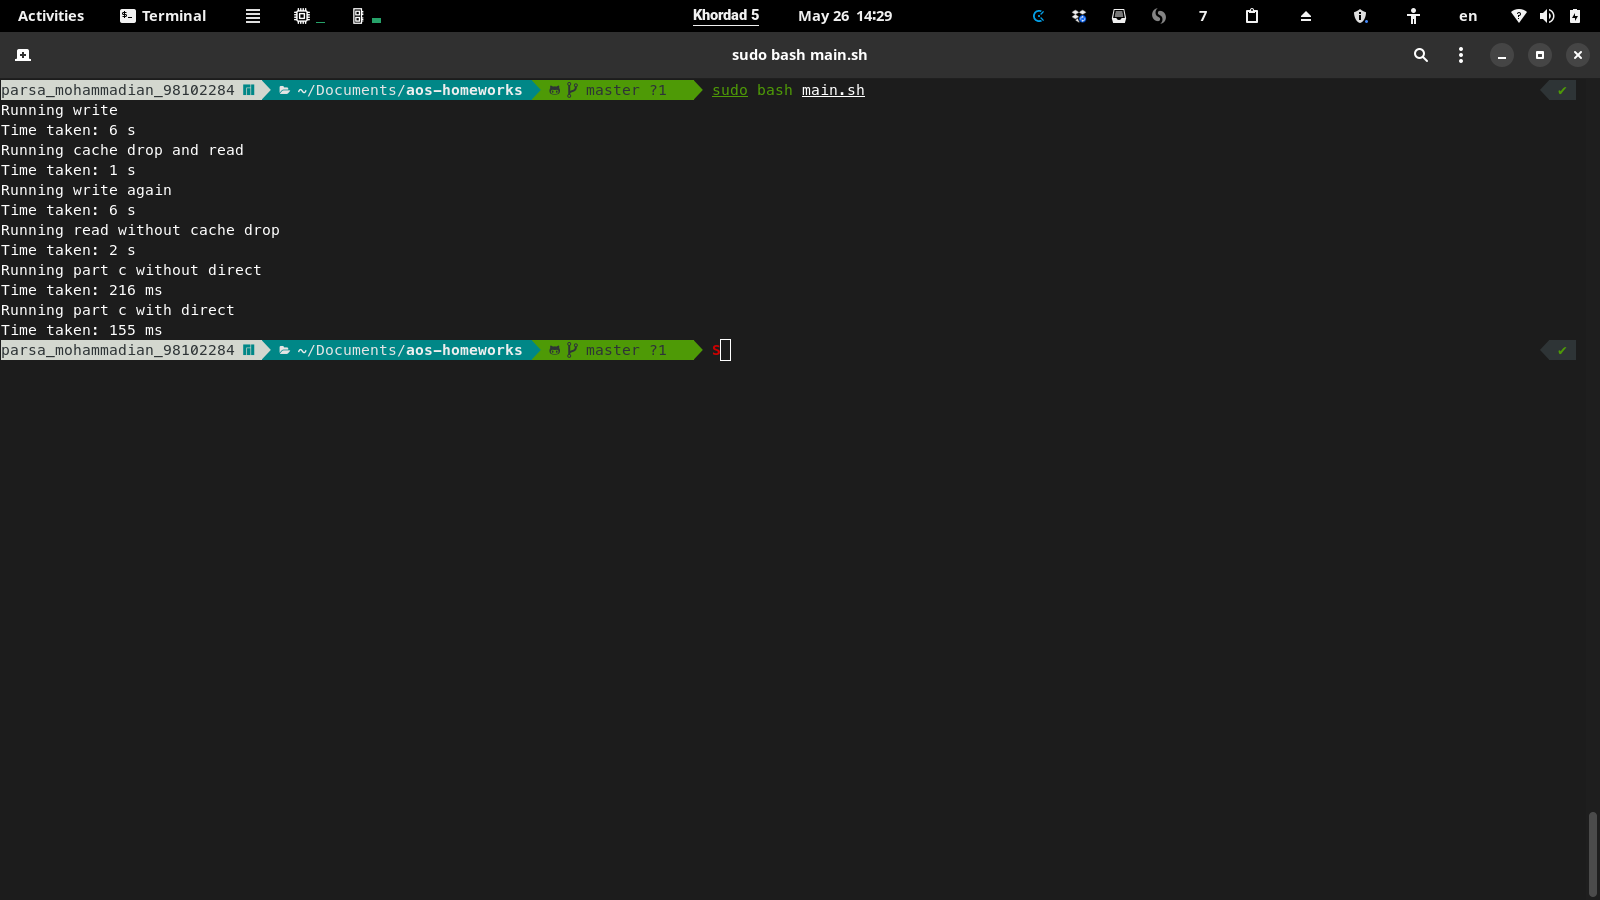
\includegraphics[width=\textwidth]{images/1.png}
\end{figure}

\subsection{}
در این قسمت برنامه اول ۶ ثانیه طول می‌کشد و برنامه دوم ۱ ثانیه. این به این معنا است 
که استفاده از فلگ 
\lr{direct}
عملیات خواندن را سریع‌تر می‌کند. دقت شود که در هر دو برنامه 
تنها زمان خواندن اندازه‌گیری شده است و در برنامه اول زمان عملیات نوشتن در نظر گرفته نشده است
تا بتوان مقایسه دقیق‌تری انجام داد.

\subsection{}
در اینجا کش را قبل از اجرای برنامه دوم پاک نمی‌کنیم. مشاهده می‌کنیم که 
برنامه اول همان ۶ ثانیه زمان برده است و برنامه دوم با وجود اینکه 
\lr{direct I/O}
است و نباید وابستگی به کش داشته باشد، ۲ ثانیه زمان می‌برد. 
به صورت کلی انگار با پاک نکردن کش، 
\lr{direct I/O}
زمان بیشتری طول می‌کشد. 

\subsection{}
در این قسمت مشاهده می‌کنیم که نوشتن با استفاده از کش 
۲۱۶ میلی ثانیه 
و نوشتن به صورت مستقیم ۱۵۵ میلی ثانیه طول می‌کشد.
نتیجه می‌گیریم که نوشتن به صورت 
\lr{direct}
سریع‌تر است ولی تاثیر آن کمتر از خواندن است. به عبارت دیگر تاثیر 
\lr{page cache}
در خواندن بیشتر مشاهده می‌شود.

\section{}
\subsection{}
\subsection{}
\subsection{}
\subsection{}
\subsection{}

\section{}
\subsection{}
\subsection{}
\subsection{}
\subsection{}
\subsection{}

\end{document}